\usetikzlibrary{arrows, positioning}

\begin{frame}
  \frametitle{Source Separation to Sequential Prediction}
  \begin{block}{From Vertical to Horizontal Analysis}
    \begin{itemize}
      \item Source separation looks at dependencies between frequencies \textbf{within a slice}, i.e. vertical analysis.
      \item Temporal correlations can be exploited to observe dependencies \textbf{between slices}, i.e. horizontal analysis.
    \end{itemize}
  \end{block}
  \begin{center}
    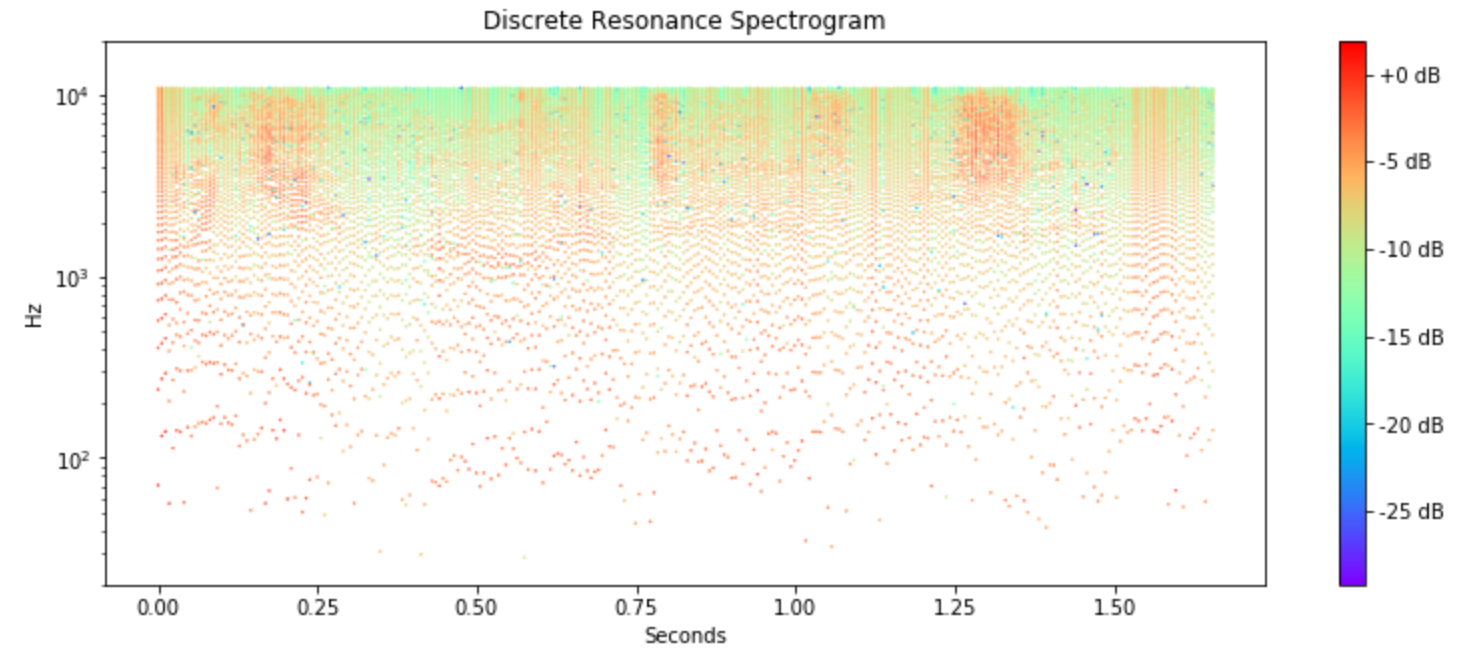
\includegraphics[width=0.8\textwidth]{images/padeogram-wide.png}
  \end{center}
\end{frame}

\begin{frame}
  \frametitle{Boundary Entropy Segmentation}
  \begin{block}{Boundary Entropy}
    \begin{itemize}
      \item Online chunking according to \textbf{pairwise sequential} regularities in order to compress a stream of symbols
      \item \textbf{Unexpectedness}: current symbol is relatively more rare
      \item \textbf{Uncertainty}: current symbol has more options to follow
    \end{itemize}
  \end{block}
  \begin{center}
    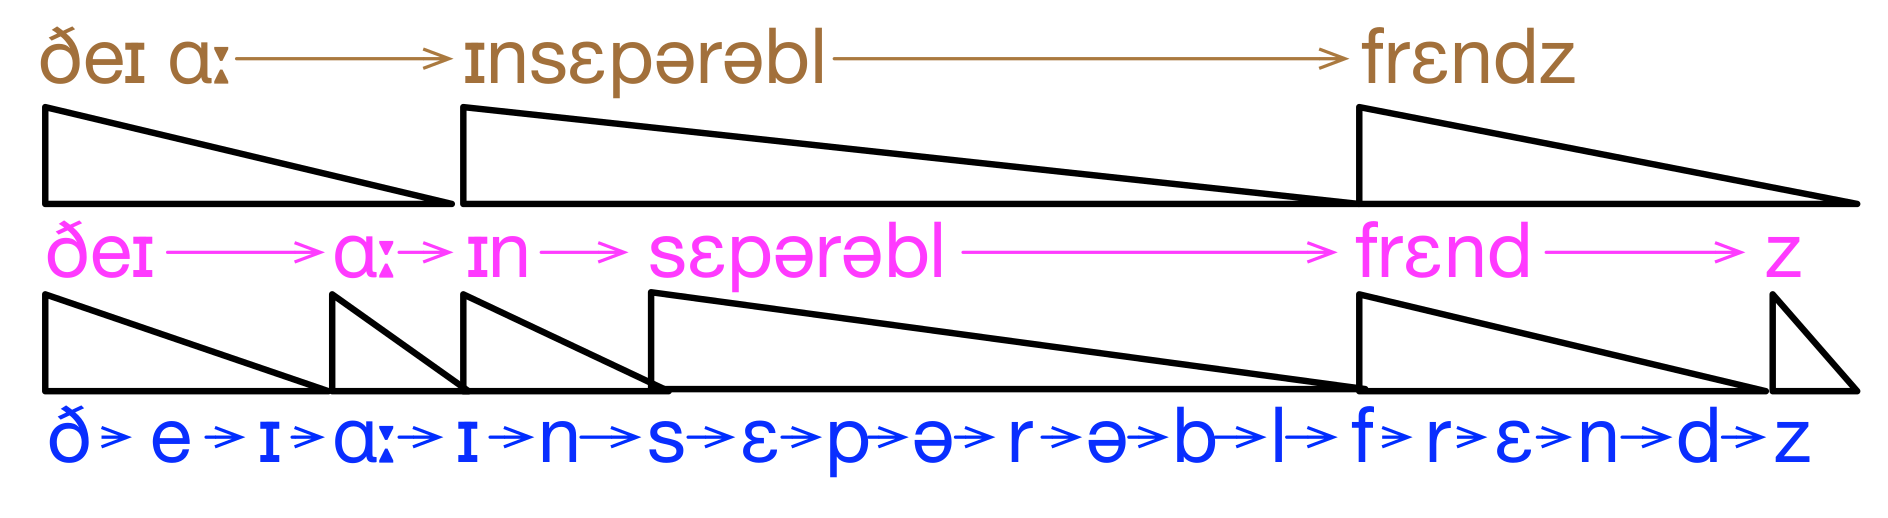
\includegraphics[width=0.9\textwidth]{images/phonetic-sequential-memory.png}
  \end{center}
\end{frame}

\begin{frame}
  \frametitle{Sequence vs Network Interpretation of BES}
  \begin{columns}
    \begin{column}{0.5\textwidth}
      \begin{block}{Sequence Interpretation}
        \begin{center}
          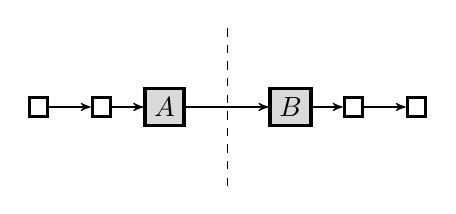
\begin{tikzpicture}[>= stealth', auto, scale=0.8]
            \tikzstyle{node}=[rectangle, very thick, draw=black]

            \node[node, fill=black!15] at (0,0) (A) {$A$};
            \node[node, fill=black!15] at (2,0) (B) {$B$};
            \node[node] (X1) at (-2,0) {};
            \node[node] (X2) at (-1,0) {};
            \node[node] (Y1) at (3,0) {};
            \node[node] (Y2) at (4,0) {};

            \path (X1) edge[->] (X2);
            \path (X2) edge[->] (A);
            \path (A) edge[->] (B);
            \path (B) edge[->] (Y1);
            \path (Y1) edge[->] (Y2);

            \draw[dashed] (1,1.25) -- (1,-1.25);

          \end{tikzpicture}
        \end{center}

        \textbf{Information Content}
        \begin{eqnarray*}\scriptstyle
          h(x) = -\log p(x)
        \end{eqnarray*}
        \textbf{Entropy}
        \begin{eqnarray*}\scriptstyle
          H(x) = -\sum_{y \in Y} p(y|x) \log p(y|x)
        \end{eqnarray*}
      \end{block}
    \end{column}
    \begin{column}{0.5\textwidth}
      \begin{block}{Network Interpretation}
        \begin{center}
          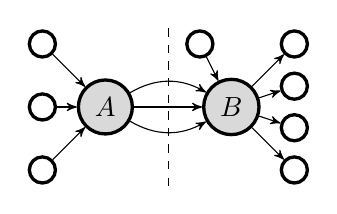
\begin{tikzpicture}[>= stealth', auto, scale=0.8]
            \tikzstyle{node}=[circle, very thick, draw=black]

            \node[node, fill=black!15] at (0,0) (A) {$A$};
            \node[node, fill=black!15] at (2,0) (B) {$B$};
            \node[node] (X2) at (-1,0) {};
            \node[node] (X1) at (-1,1) {};
            \node[node] (X3) at (-1,-1) {};
            \node[node] (Y2) at (3,1) {};
            \node[node] (Y1) at (3,0.33) {};
            \node[node] (Y3) at (3,-0.33) {};
            \node[node] (Y4) at (3, -1) {};
            \node[node] (Z) at (1.5, 1) {};

            \path (X1) edge[->] (A);
            \path (X2) edge[->] (A);
            \path (X3) edge[->] (A);
            \path (A) edge[->] (B);
            \path (A) edge[->] [bend left] (B);
            \path (A) edge[->] [bend right] (B);
            \path (Z) edge[->] (B);
            \path (B) edge[->] (Y1);
            \path (B) edge[->] (Y2);
            \path (B) edge[->] (Y3);
            \path (B) edge[->] (Y4);

            \draw[dashed] (1,1.25) -- (1,-1.25);

          \end{tikzpicture}
        \end{center}

        \textbf{In-Entropy}
        \begin{eqnarray*}\scriptstyle
          H_{in}(x) = -\sum_{y \in In(x)} p(x|y) \log p(x|y)
        \end{eqnarray*}
        \textbf{Out-Entropy}
        \begin{eqnarray*}\scriptstyle
          H_{out}(x) = -\sum_{y \in Out(x)} p(y|x) \log p(y|x)
        \end{eqnarray*}
      \end{block}
    \end{column}
  \end{columns}
\end{frame}

\begin{frame}
  \frametitle{Hierarchical Structure and Dynamics}
  \begin{columns}
    \begin{column}{0.5\textwidth}
      \begin{block}{Hierarchical Prediction}
        \begin{center}
          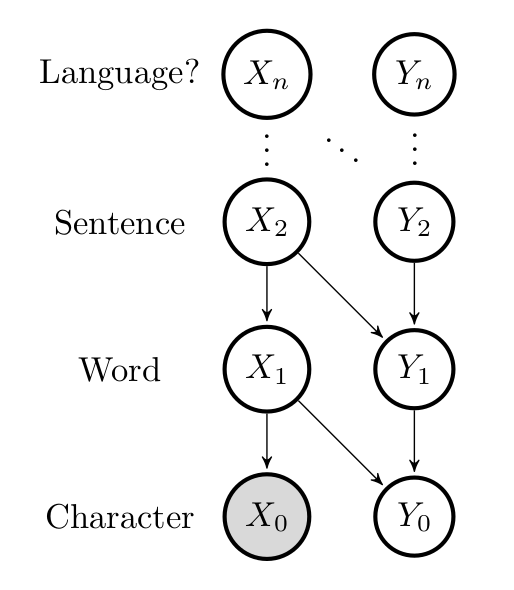
\includegraphics[width=0.97\textwidth]{images/idyot-seqmem-graph-model.png}
        \end{center}
      \end{block}
    \end{column}
    \begin{column}{0.5\textwidth}
      \begin{block}{Hierarchical Structure}
        \begin{center}
          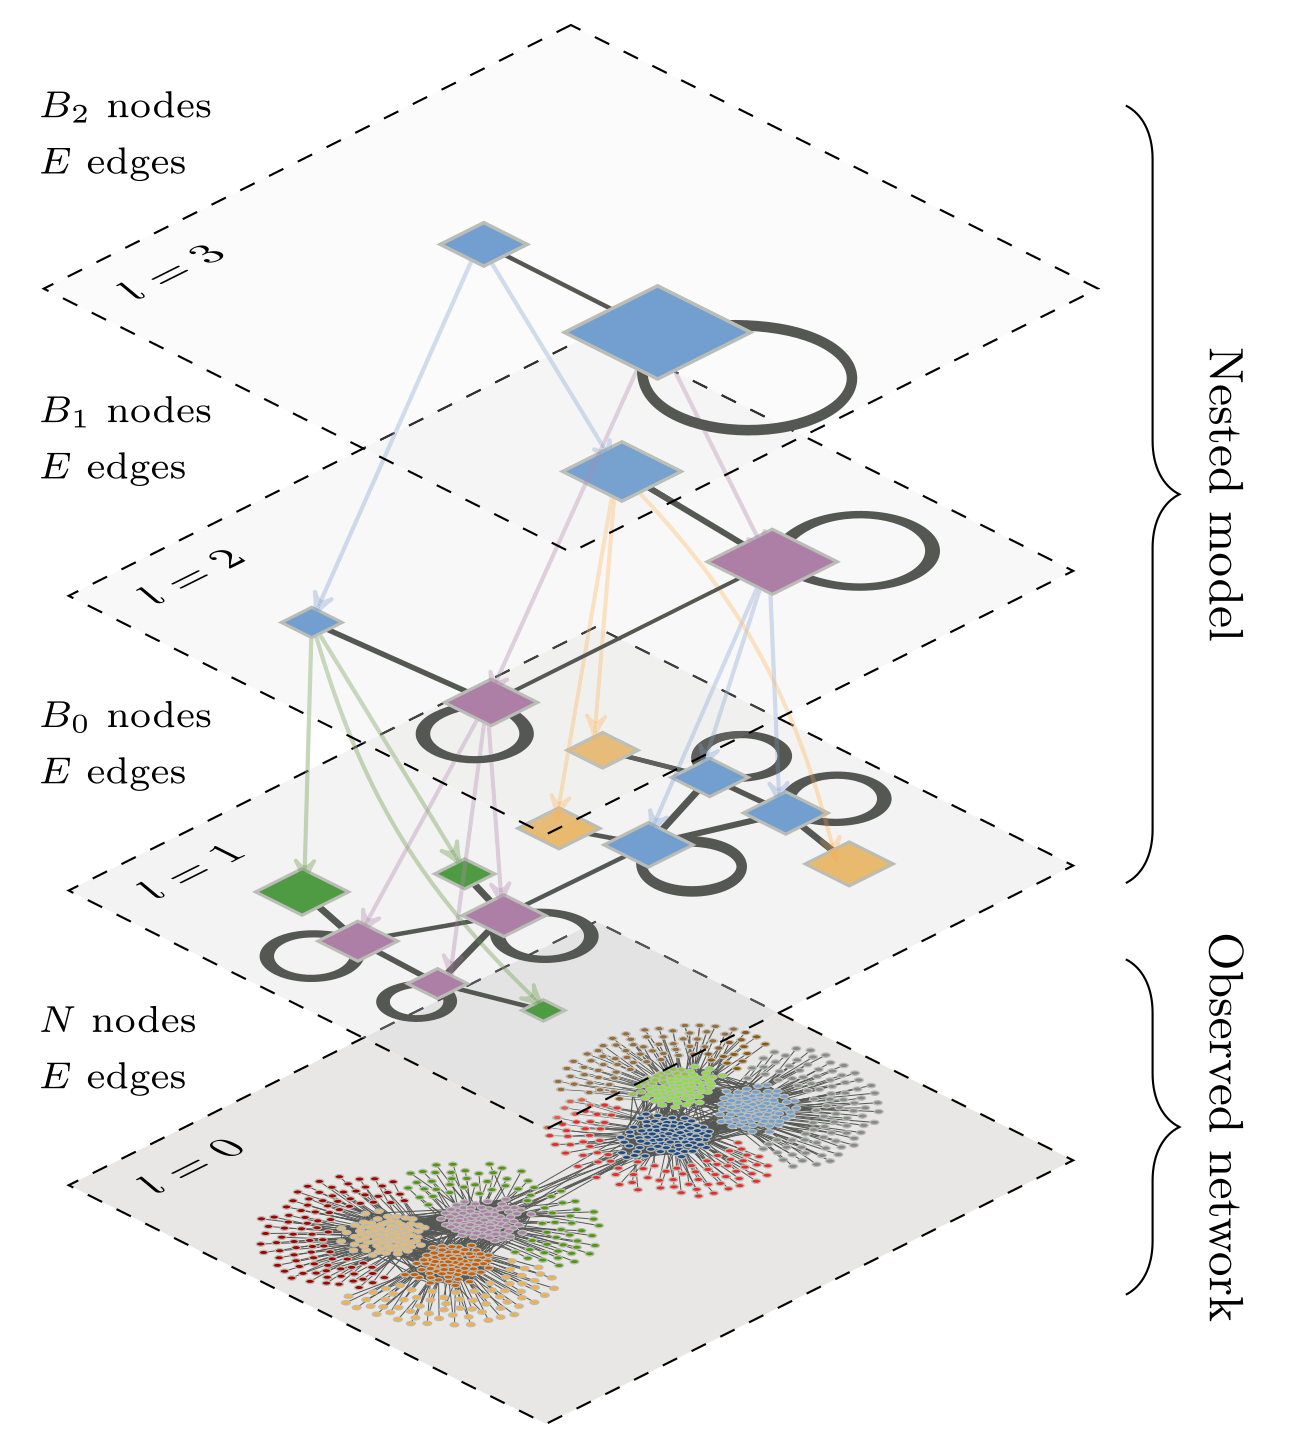
\includegraphics[width=\textwidth]{images/hierarchical-block-model.png}
        \end{center}
      \end{block}
    \end{column}
  \end{columns}
\end{frame}

\begin{frame}
  \frametitle{Information Efficiency and the MDL Principle}
  \begin{block}{Memory Consolidation}
    \begin{itemize}
      \item According to the \textbf{information efficiency} criterion of IDyOT, online boundary entropy segmentation is likely suboptimal
      \item \textbf{Offline memory consolidation} can fix some missteps that occurred online by lowering the total entropy of the model
    \end{itemize}
  \end{block}
  \begin{block}{Minimum Description Length Principle}
    \begin{itemize}
      \item $\Sigma$ (Description) = $\mathcal{L}$ (Model) + $\mathcal{S}$ (Data) (in bits)
      \item Least complex model that accurately describes the data
      \item Used for \textbf{model selection} in AIT and complex networks
    \end{itemize}
  \end{block}
\end{frame}

\begin{frame}
  \frametitle{Placement and Next Steps}
  \begin{block}{Placement of Research}
    \begin{itemize}
      \item \textbf{Online vs offline} community structure detection 
      \item \textbf{Topological vs causal} structure inference in networks
      \item \textbf{Static vs temporal} system dynamics and link prediction 
    \end{itemize}
  \end{block}
  \begin{block}{Immediate Next Steps}
    \begin{itemize}
      \item Causal network topology \textbf{inference} and sequence prediction through boundary entropy segmentation
      \item Memory \textbf{consolidation} based on MDL principle for networks
    \end{itemize}
  \end{block}
\end{frame}

\begin{frame}
  \frametitle{Applications and Future Work}
  \begin{block}{Applications}
    \begin{itemize}
      \item Voice extraction in noisy industrial environments
      \item Pitch tracking and pitch to midi
      \item Straight up compression
    \end{itemize}
  \end{block}
  \begin{block}{Future Work}
    \begin{itemize}
      \item Information-theoretic \textbf{categorization} of frequency space
      \item Robot route finding structure
      \item 
    \end{itemize}
  \end{block}
\end{frame}
